\chapter{Results}
\label{chap:results}

% overview
% what do the results show

\section{Experimental Setup}

% Hardware stats
% random generator seed based to recreate instances
% list experiments


\section{Assembly for Target Size}

\begin{figure}
	\centering
	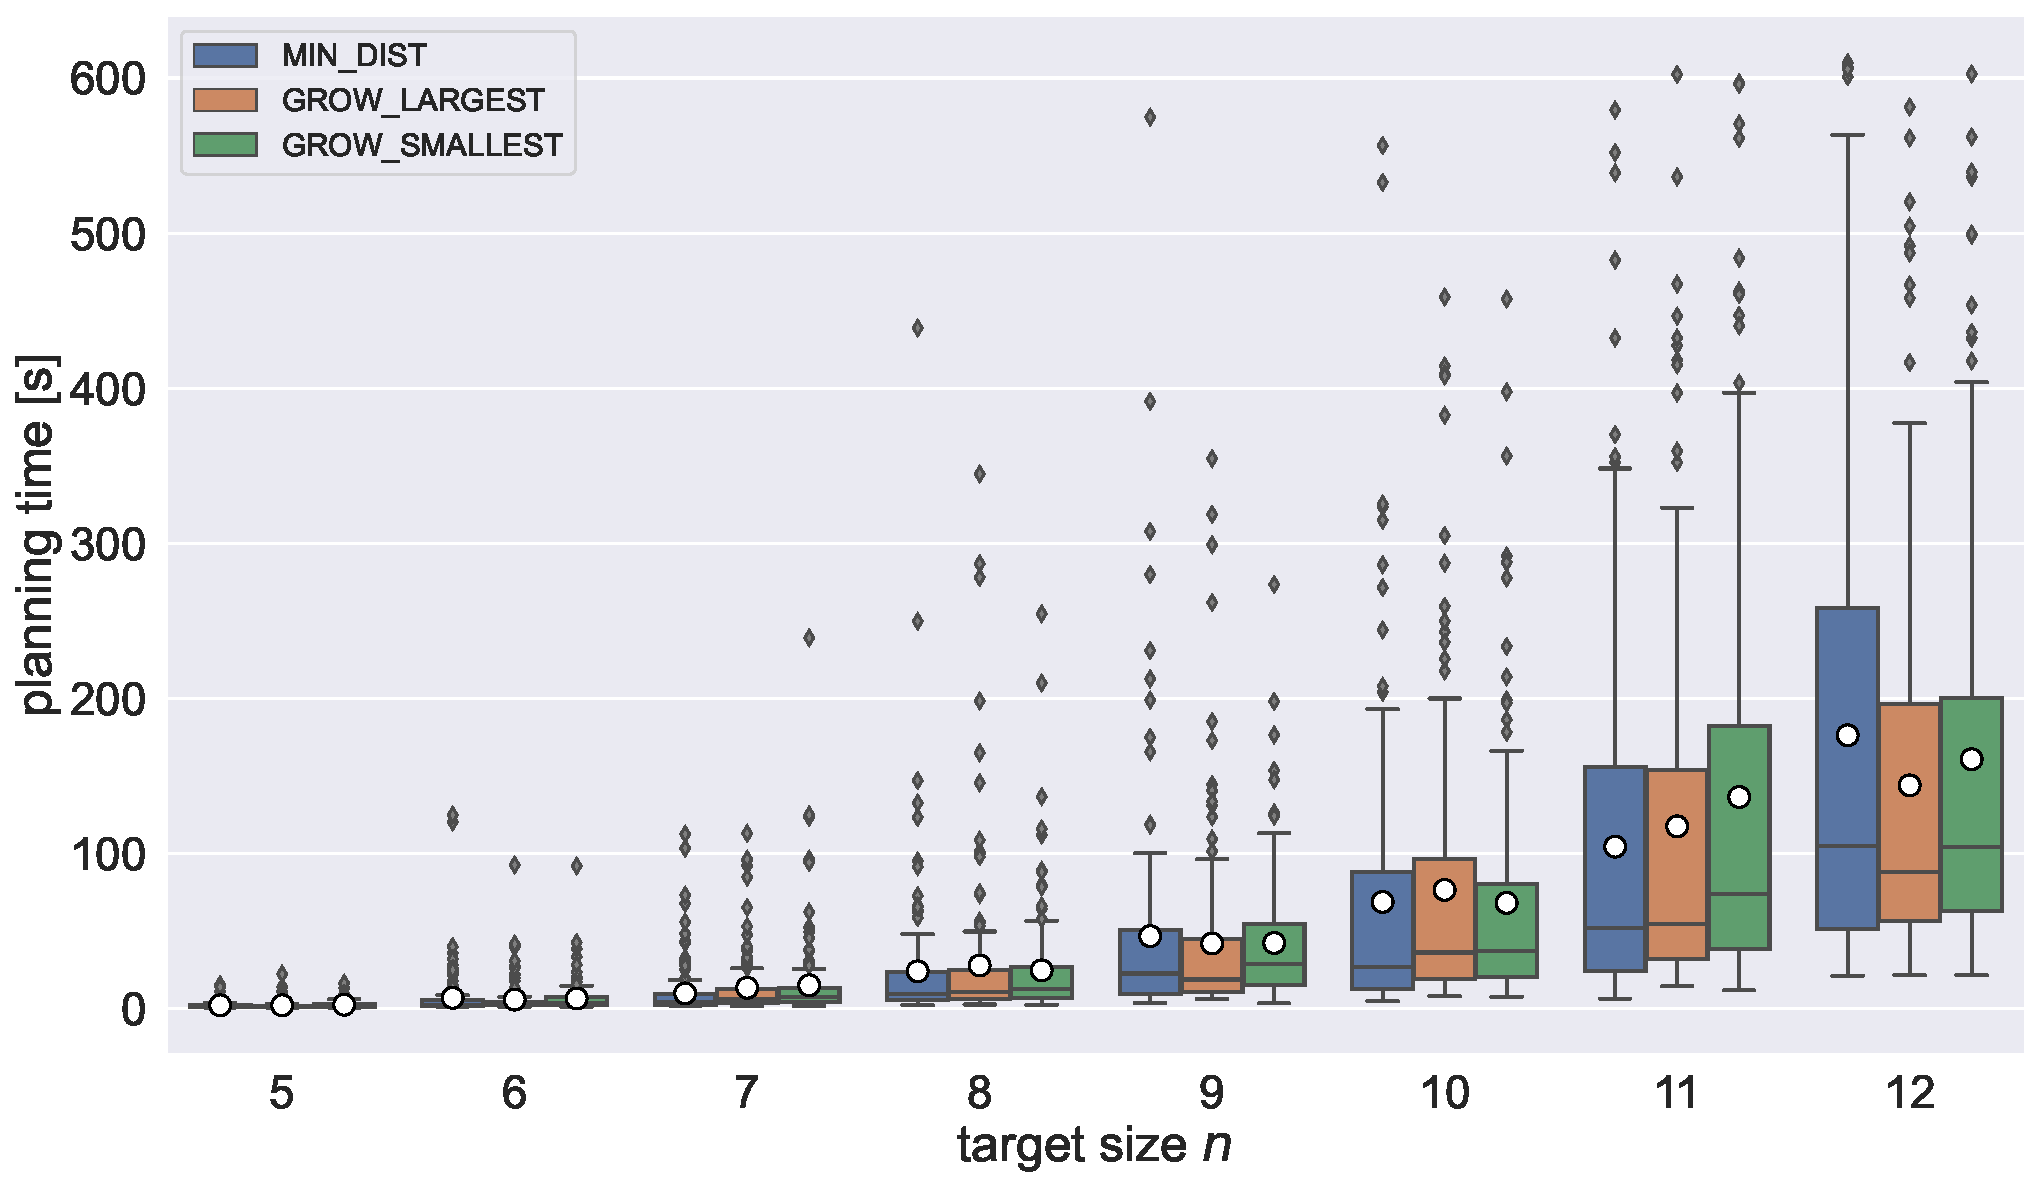
\includegraphics[width=0.9\textwidth]{figures/plots/AFN_time.pdf}
	\caption[]{}
	\label{fig:AFN_time}
\end{figure}

\begin{figure}
	\centering
	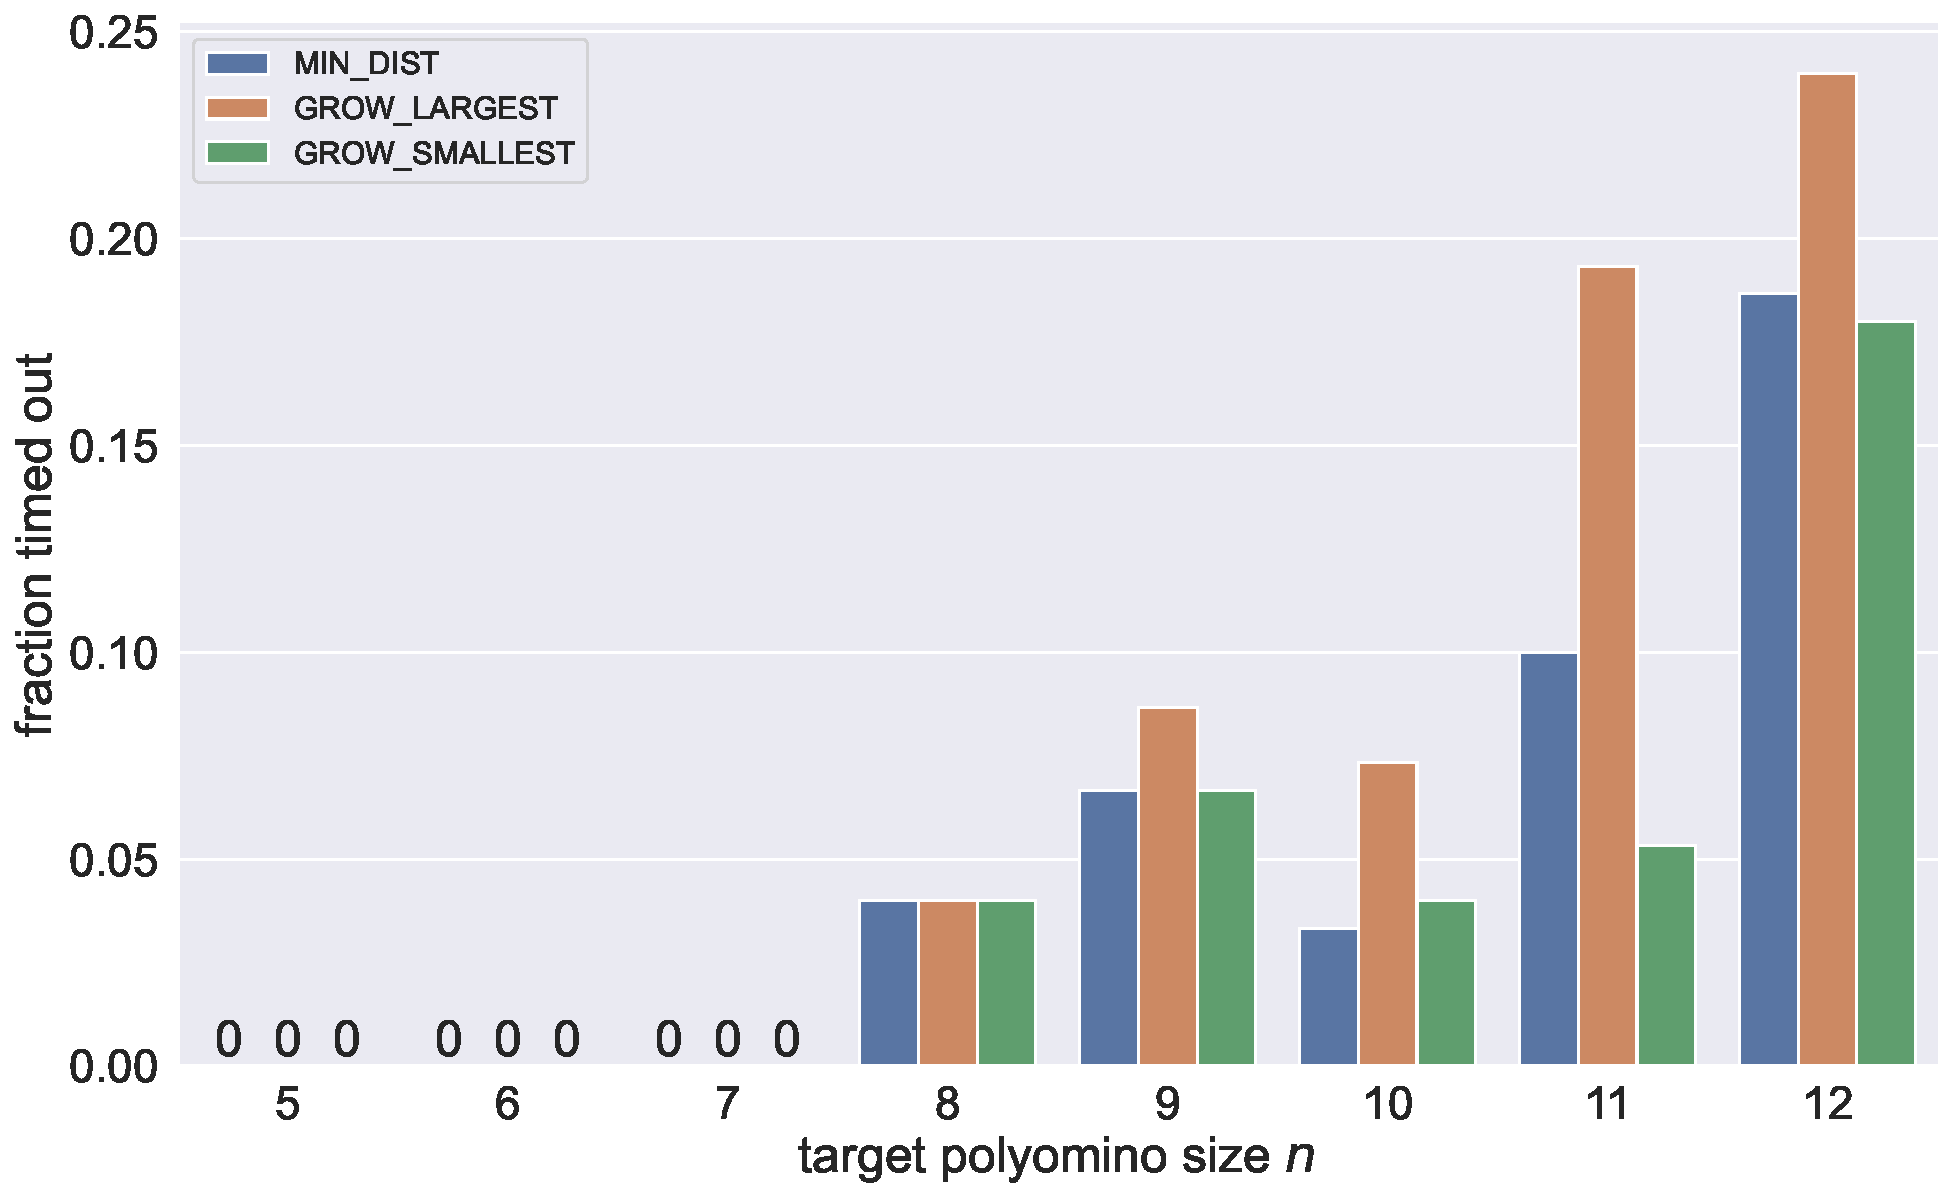
\includegraphics[width=0.9\textwidth]{figures/plots/AFN_timeout.pdf}
	\caption[]{}
	\label{fig:AFN_timeout}
\end{figure}

\begin{figure}
	\centering
	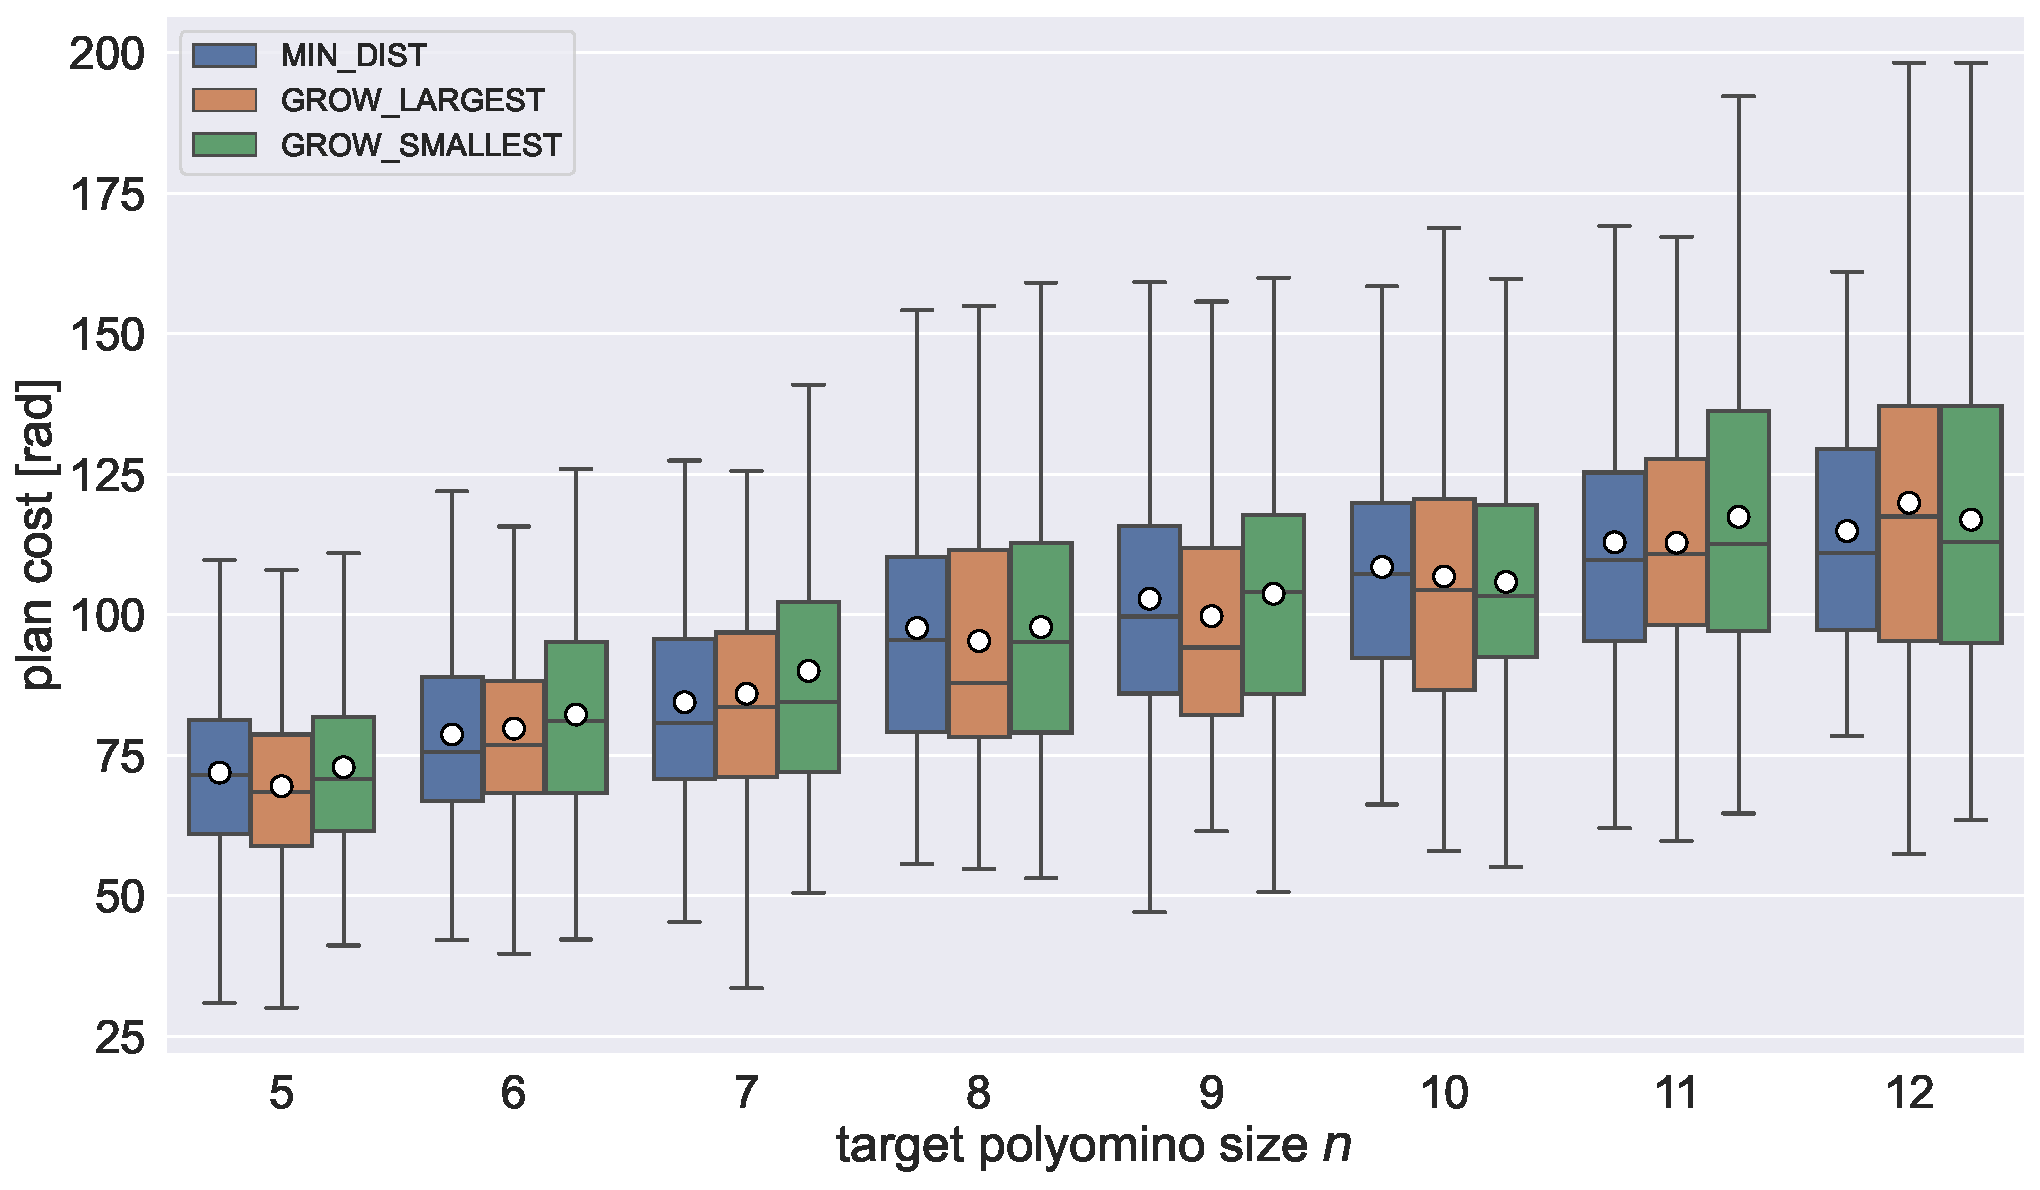
\includegraphics[width=0.9\textwidth]{figures/plots/AFN_cost.pdf}
	\caption[]{}
	\label{fig:AFN_cost}
\end{figure}

\begin{figure}
	\centering
	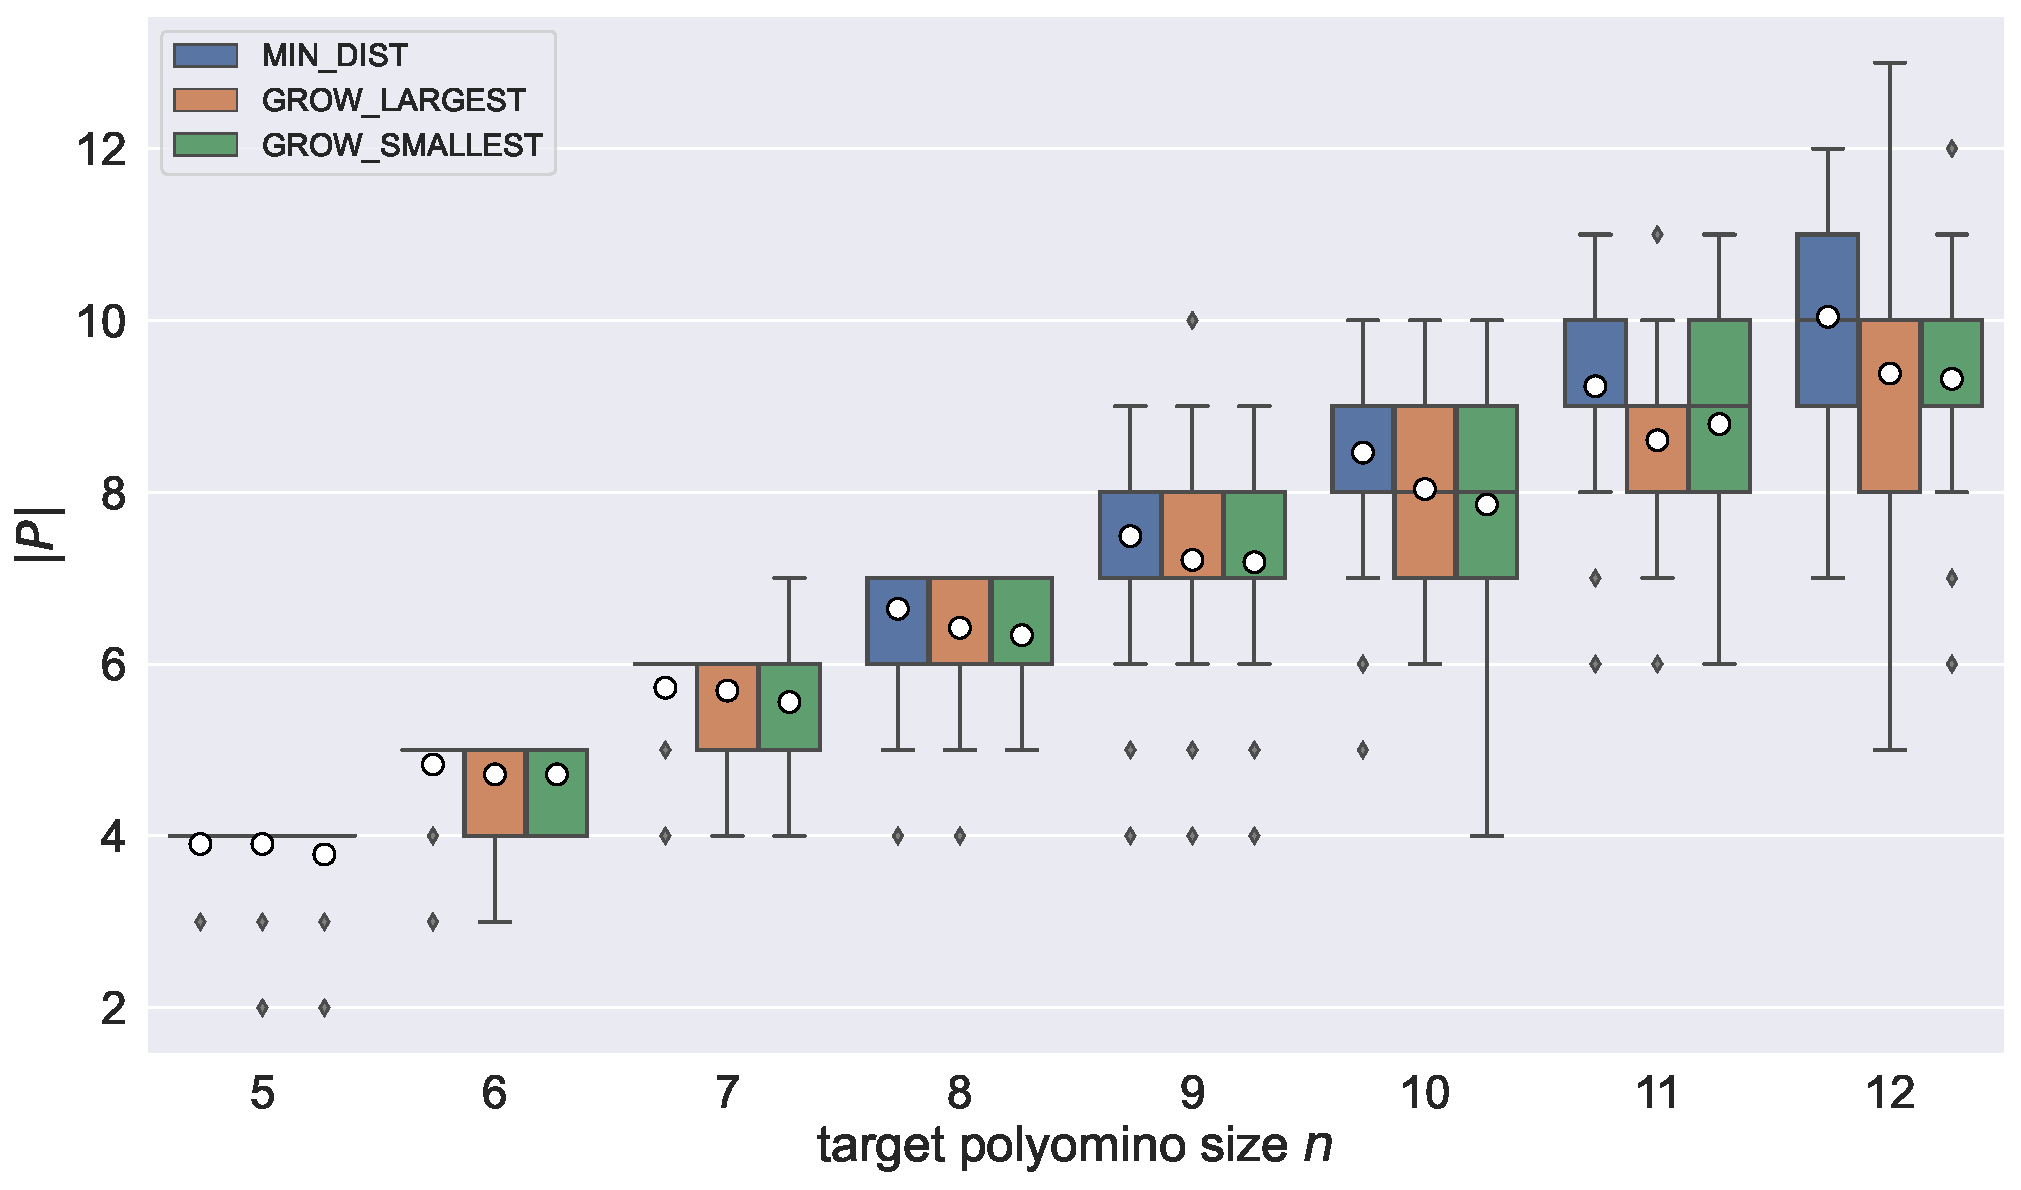
\includegraphics[width=0.9\textwidth]{figures/plots/AFN_ltg.pdf}
	\caption[]{}
	\label{fig:AFN_ltg}
\end{figure}

\begin{figure}
	\centering
	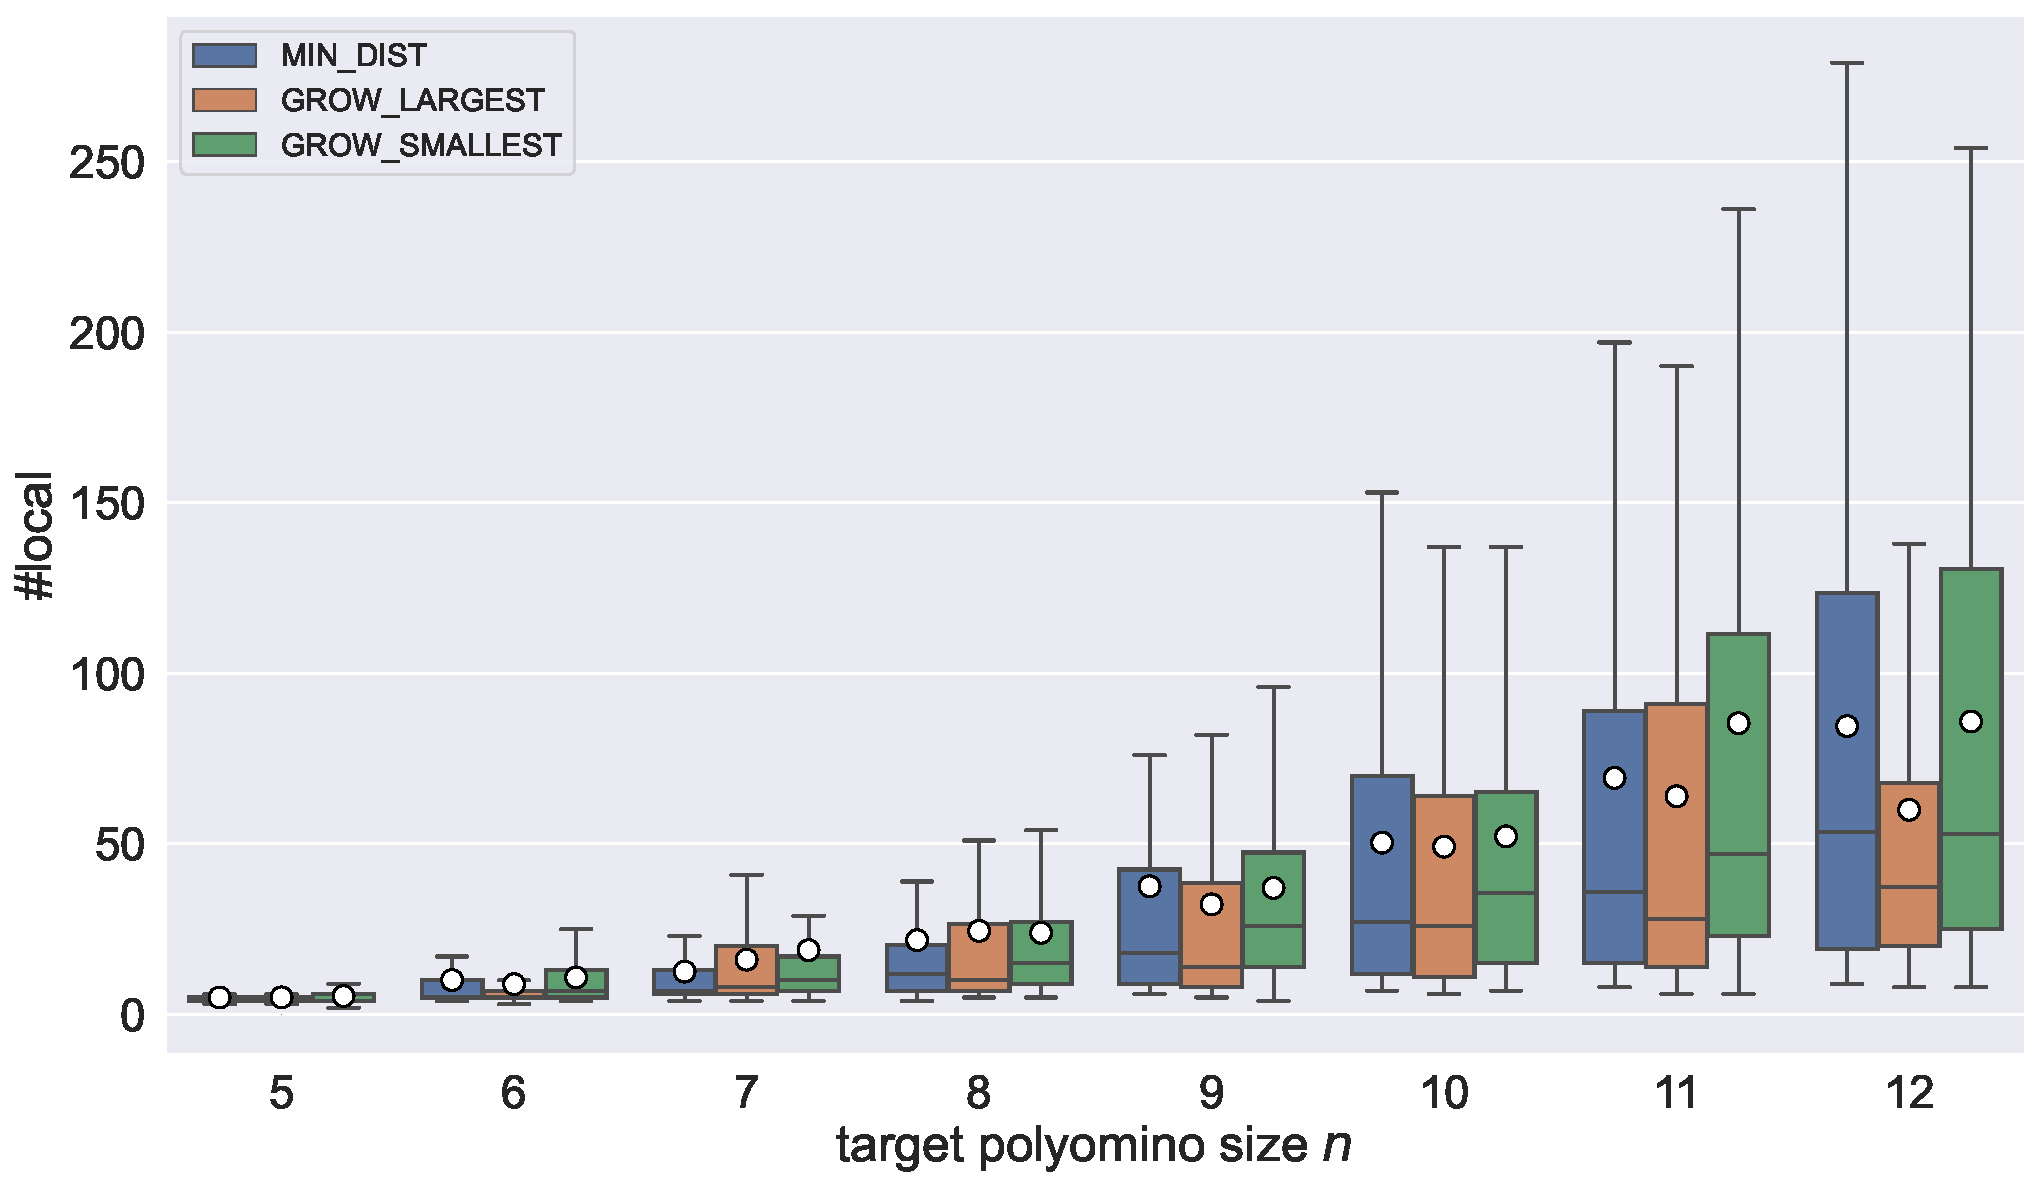
\includegraphics[width=0.9\textwidth]{figures/plots/AFN_nlocal.pdf}
	\caption[]{}
	\label{fig:AFN_nlocal}
\end{figure}

\begin{figure}
	\centering
	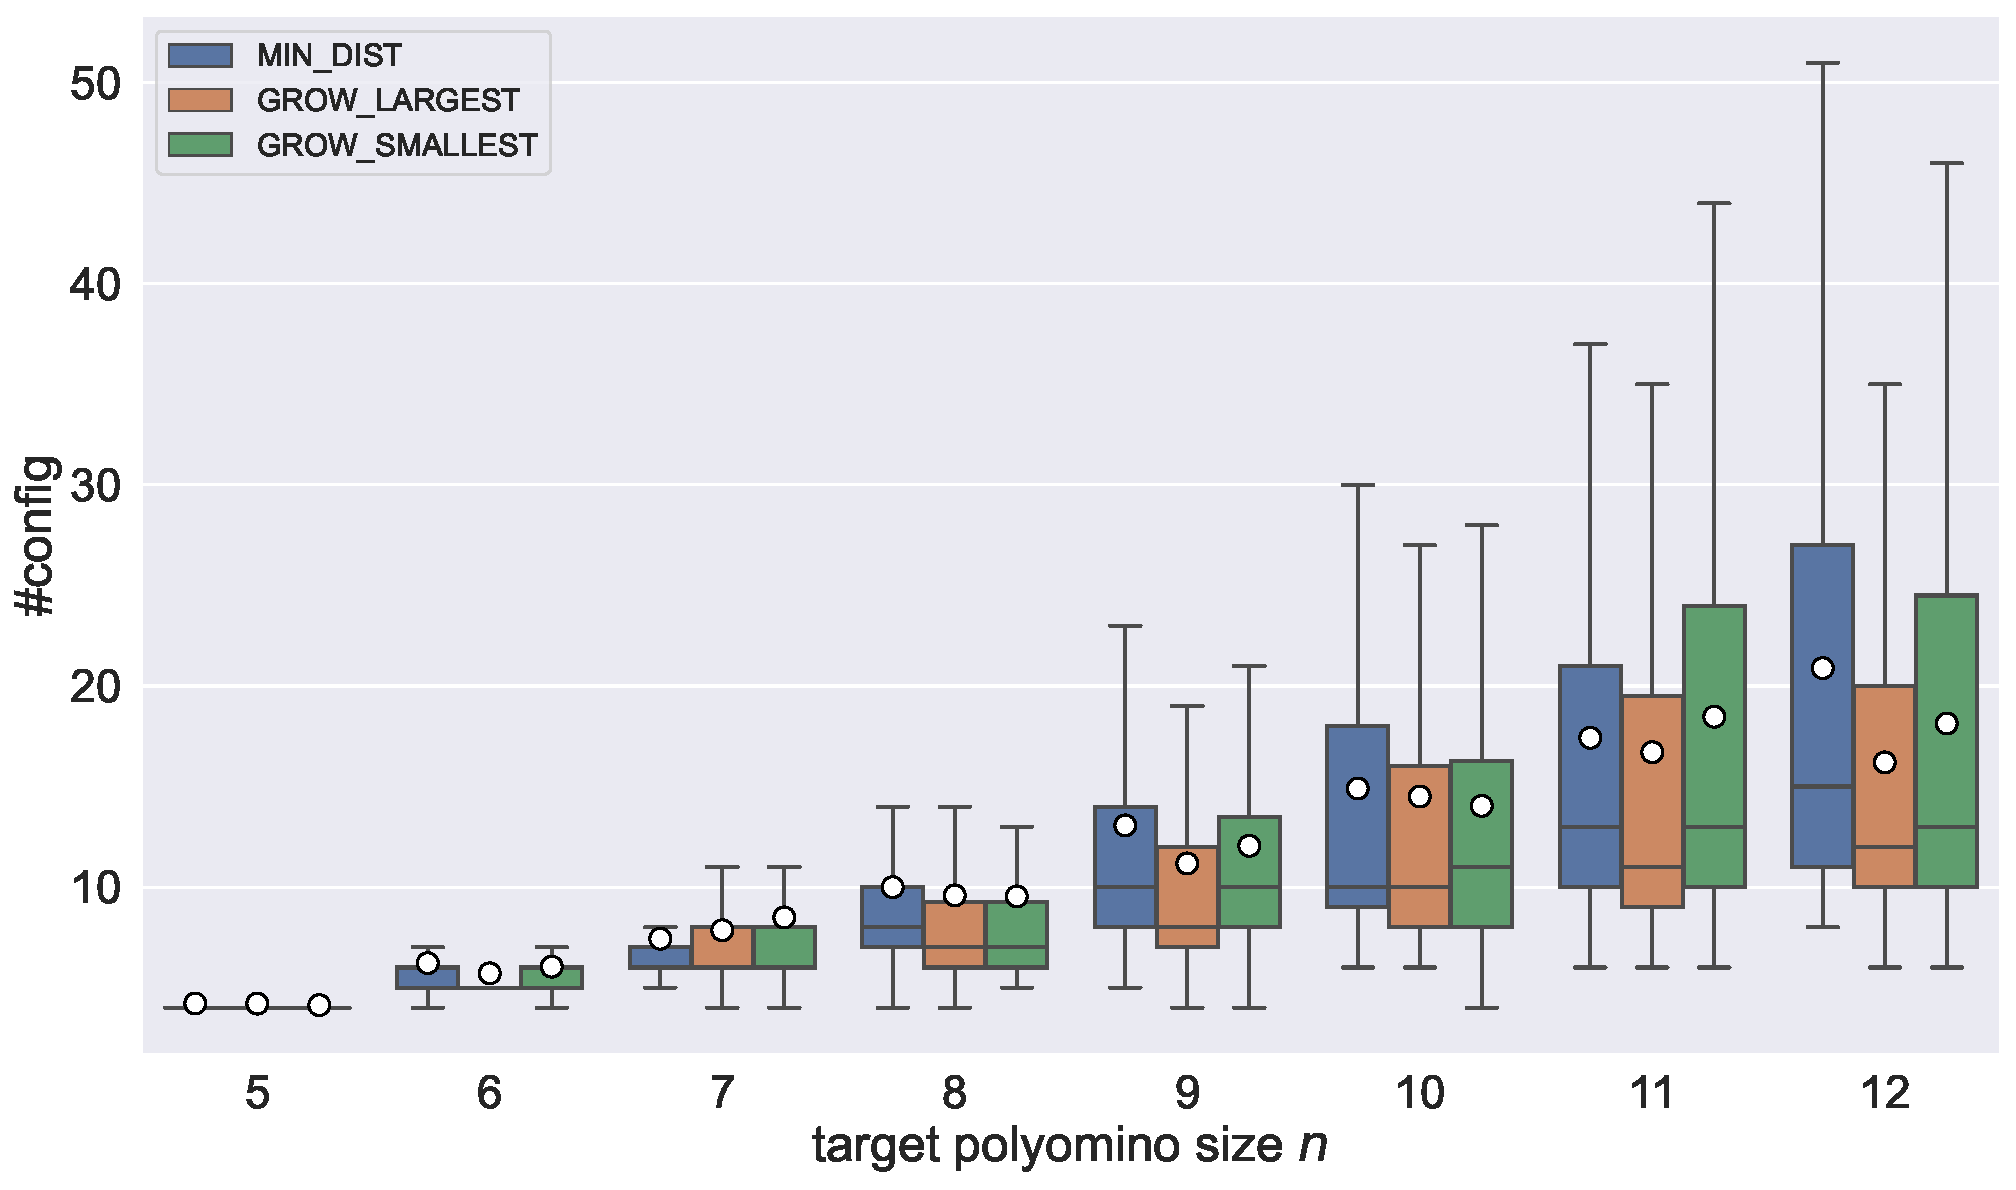
\includegraphics[width=0.9\textwidth]{figures/plots/AFN_nconfig.pdf}
	\caption[]{}
	\label{fig:AFN_nconfig}
\end{figure}




\section{Assembly for Target Shape}

\begin{figure}
	\centering
	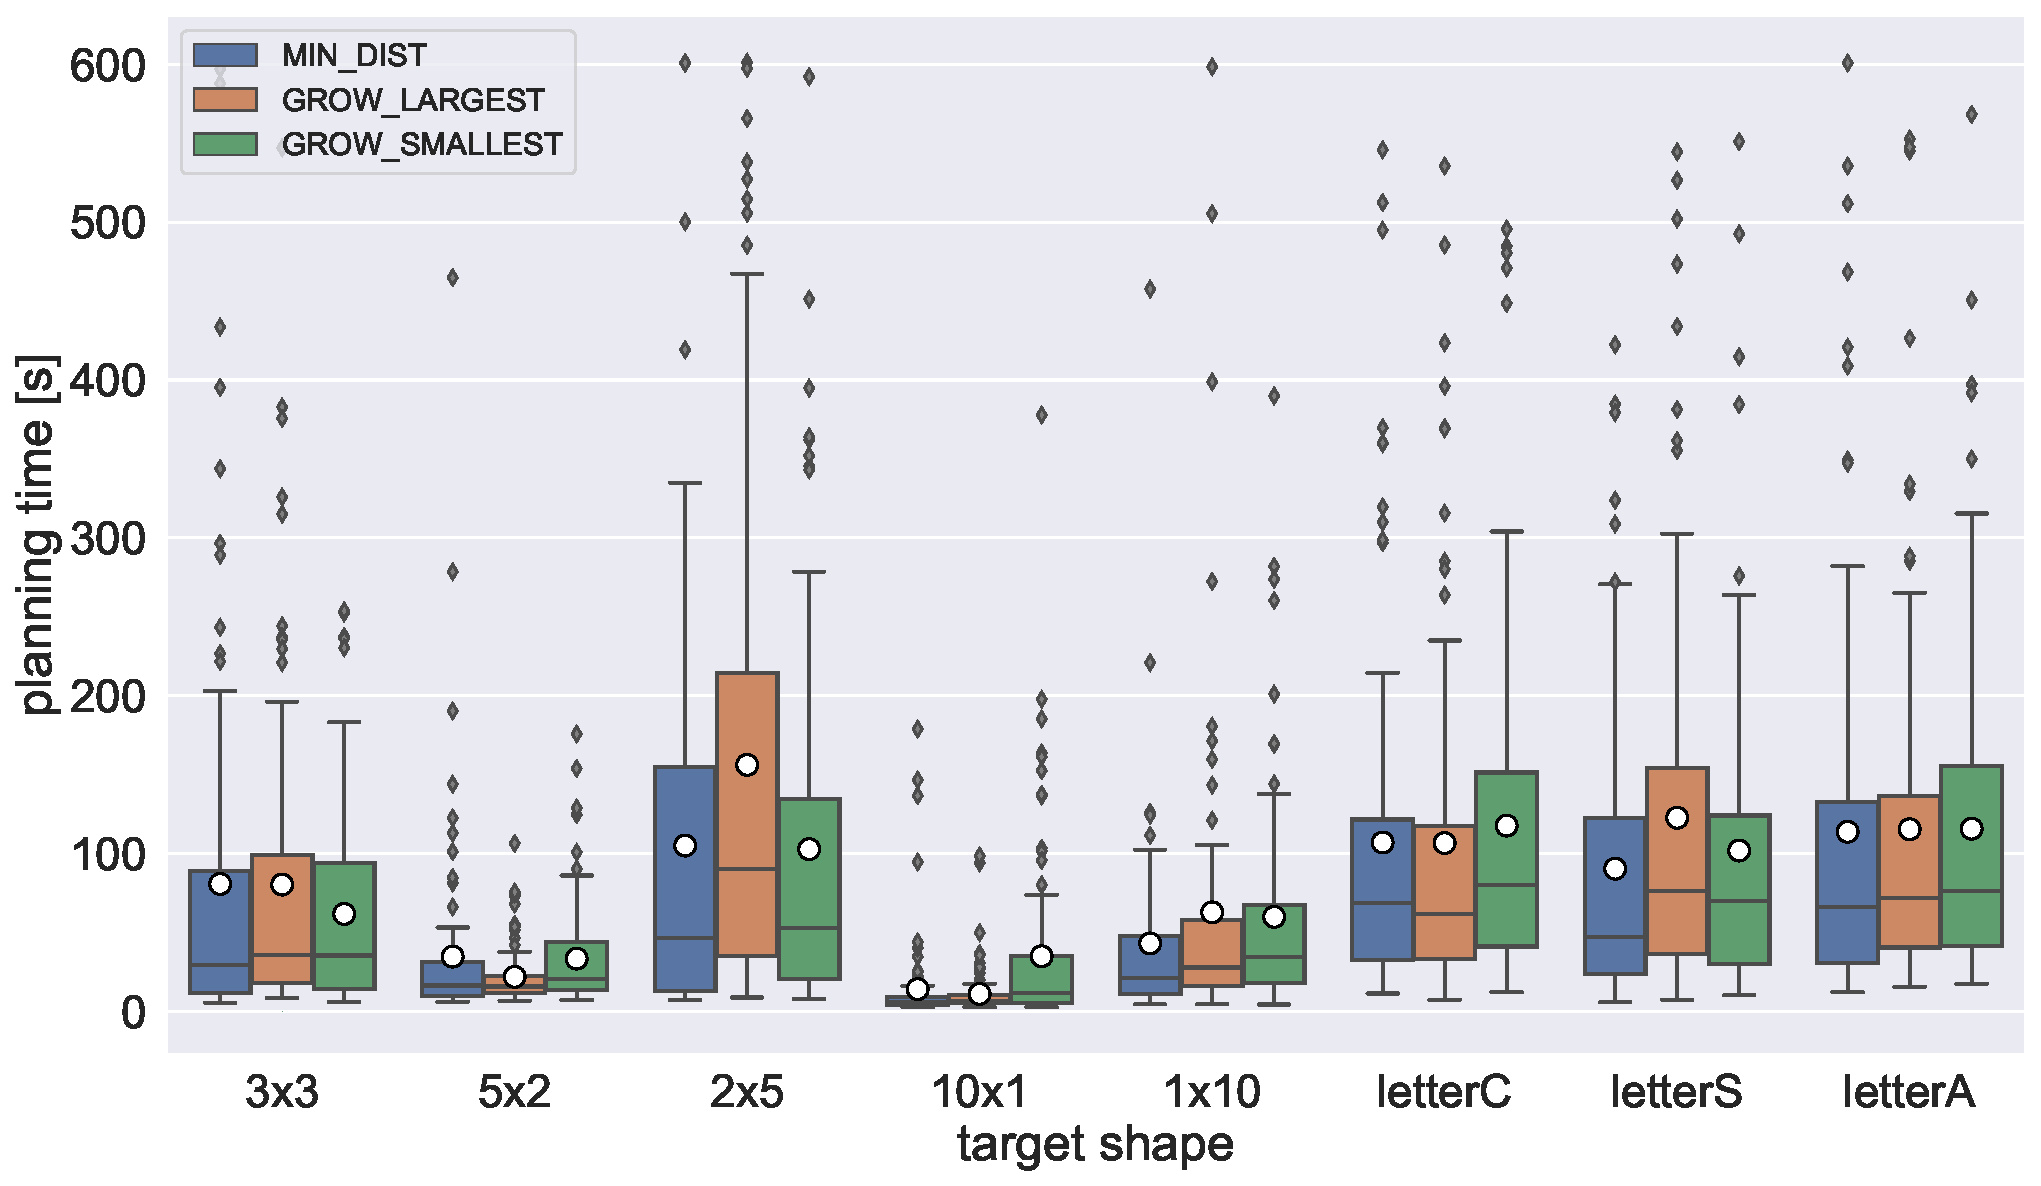
\includegraphics[width=0.9\textwidth]{figures/plots/AFTS_time.pdf}
	\caption[]{}
	\label{fig:AFTS_time}
\end{figure}

\begin{figure}
	\centering
	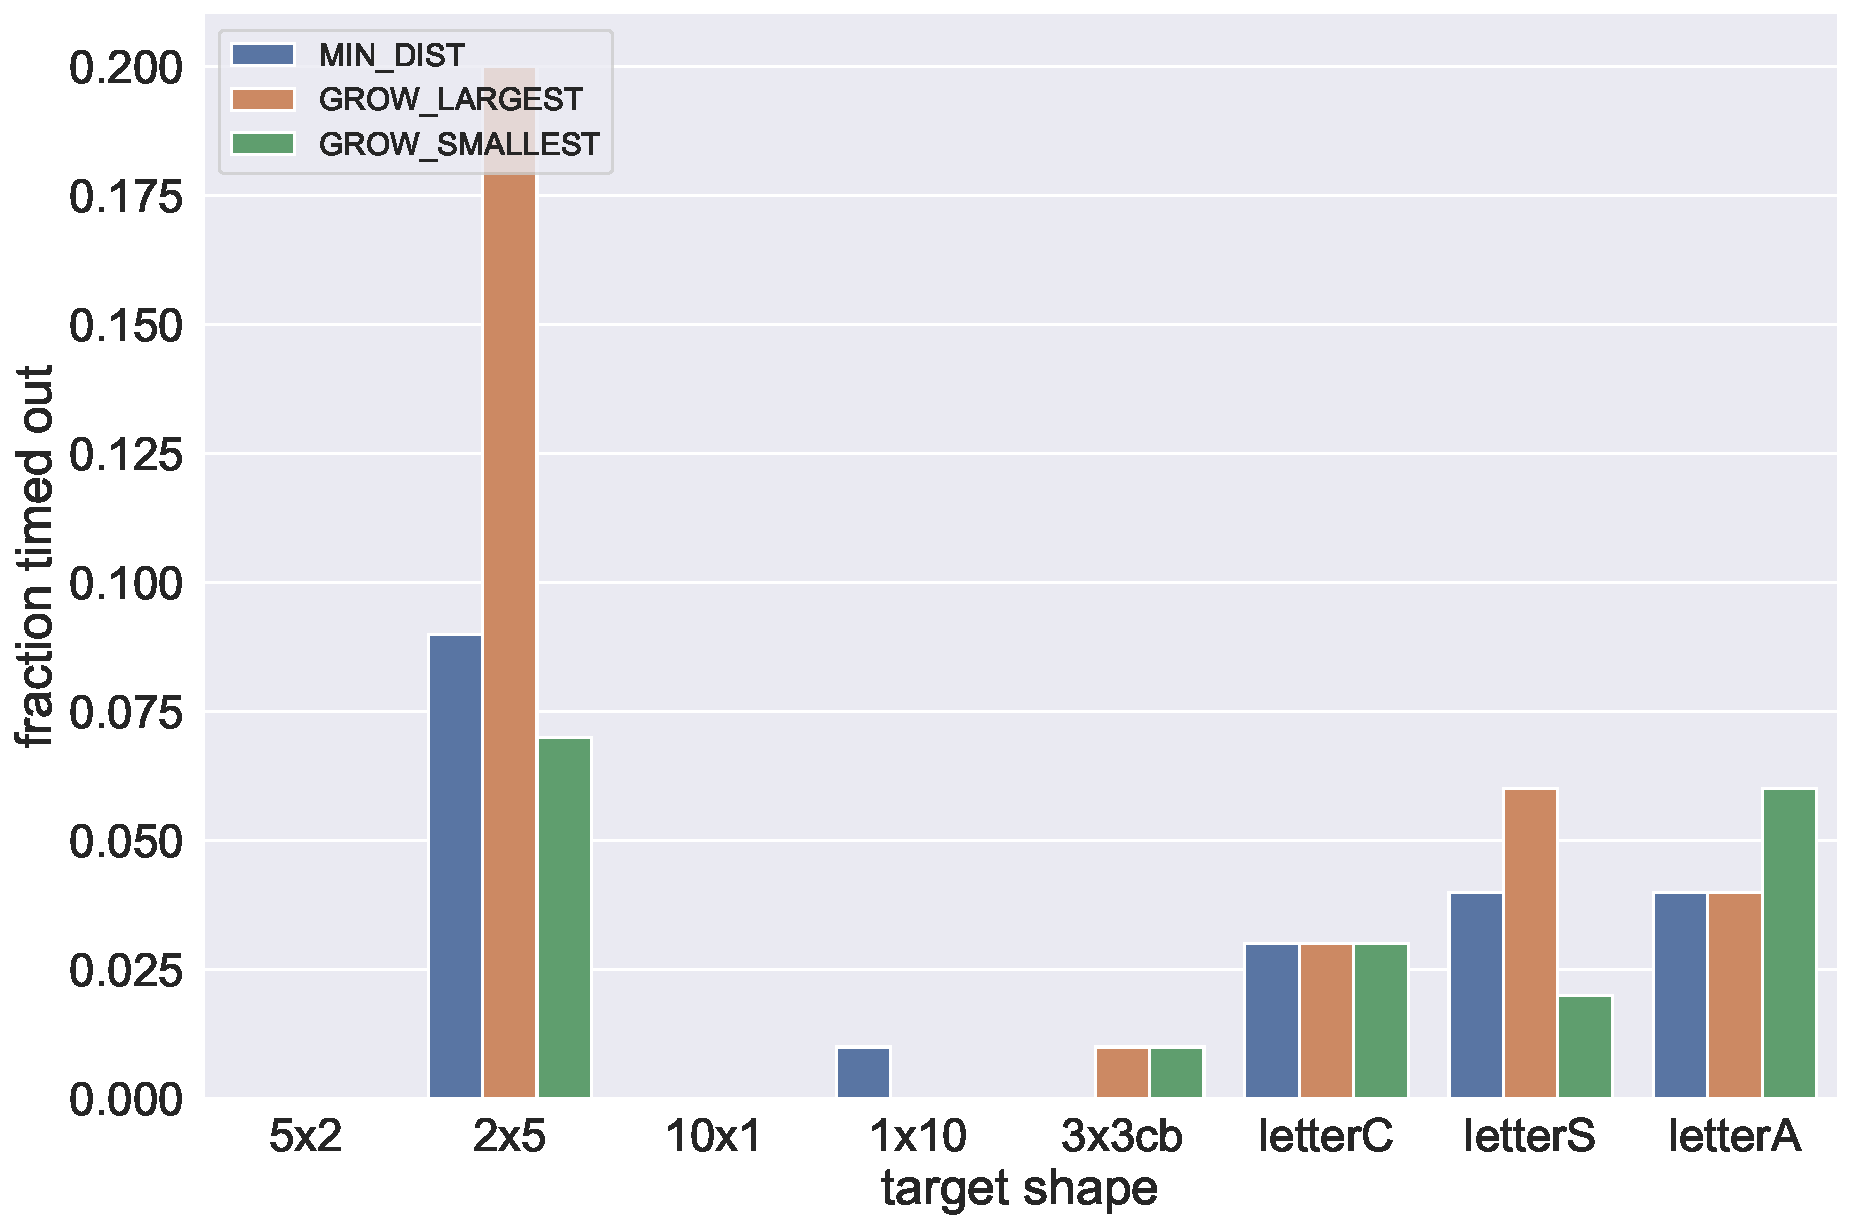
\includegraphics[width=0.9\textwidth]{figures/plots/AFTS_timeout.pdf}
	\caption[]{}
	\label{fig:AFTS_timeout}
\end{figure}




\section{Assembly for Workspace Size}

\begin{figure}
	\centering
	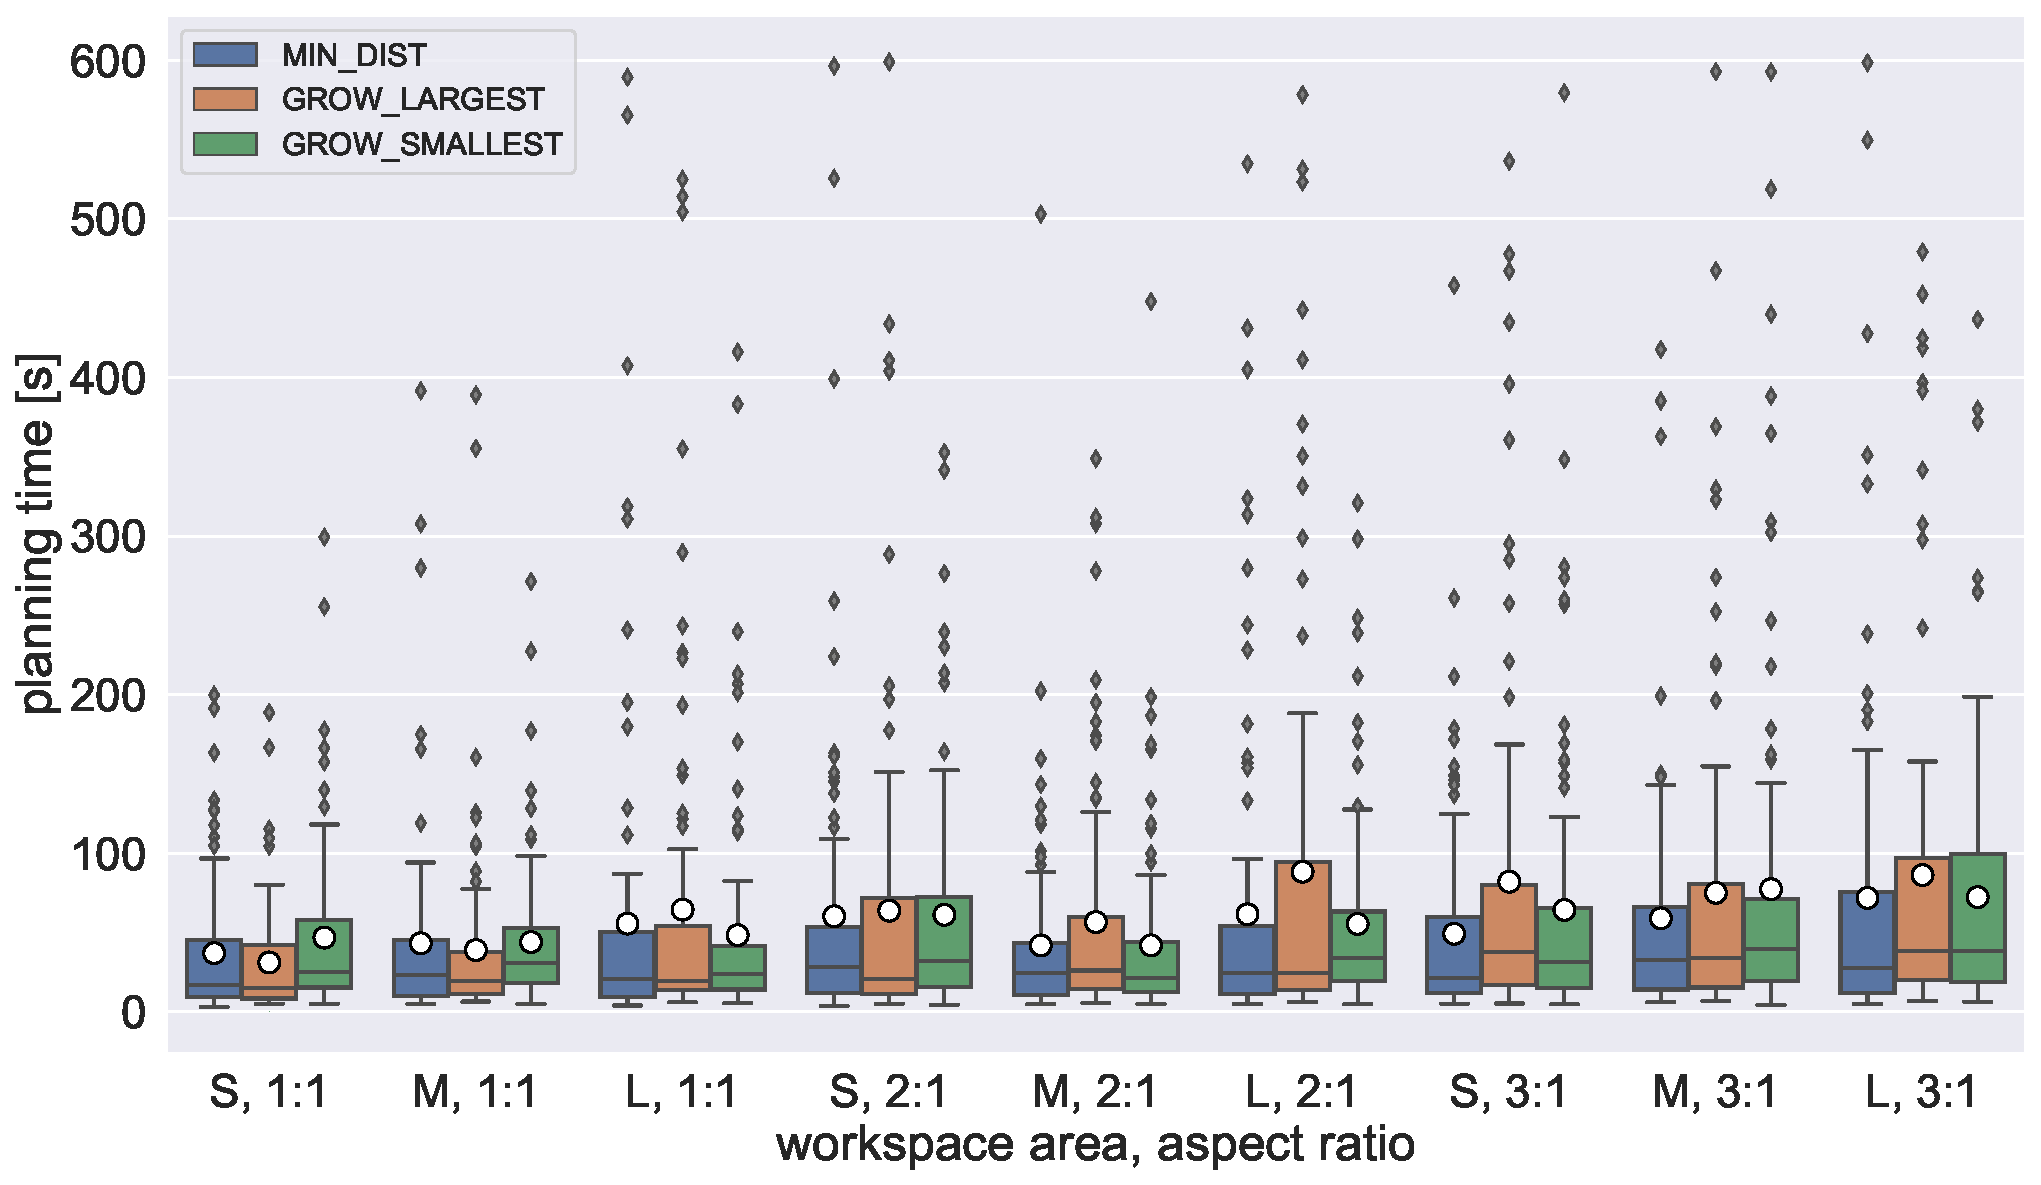
\includegraphics[width=0.9\textwidth]{figures/plots/AFBS_time.pdf}
	\caption[]{}
	\label{fig:AFBS_time}
\end{figure}

\begin{figure}
	\centering
	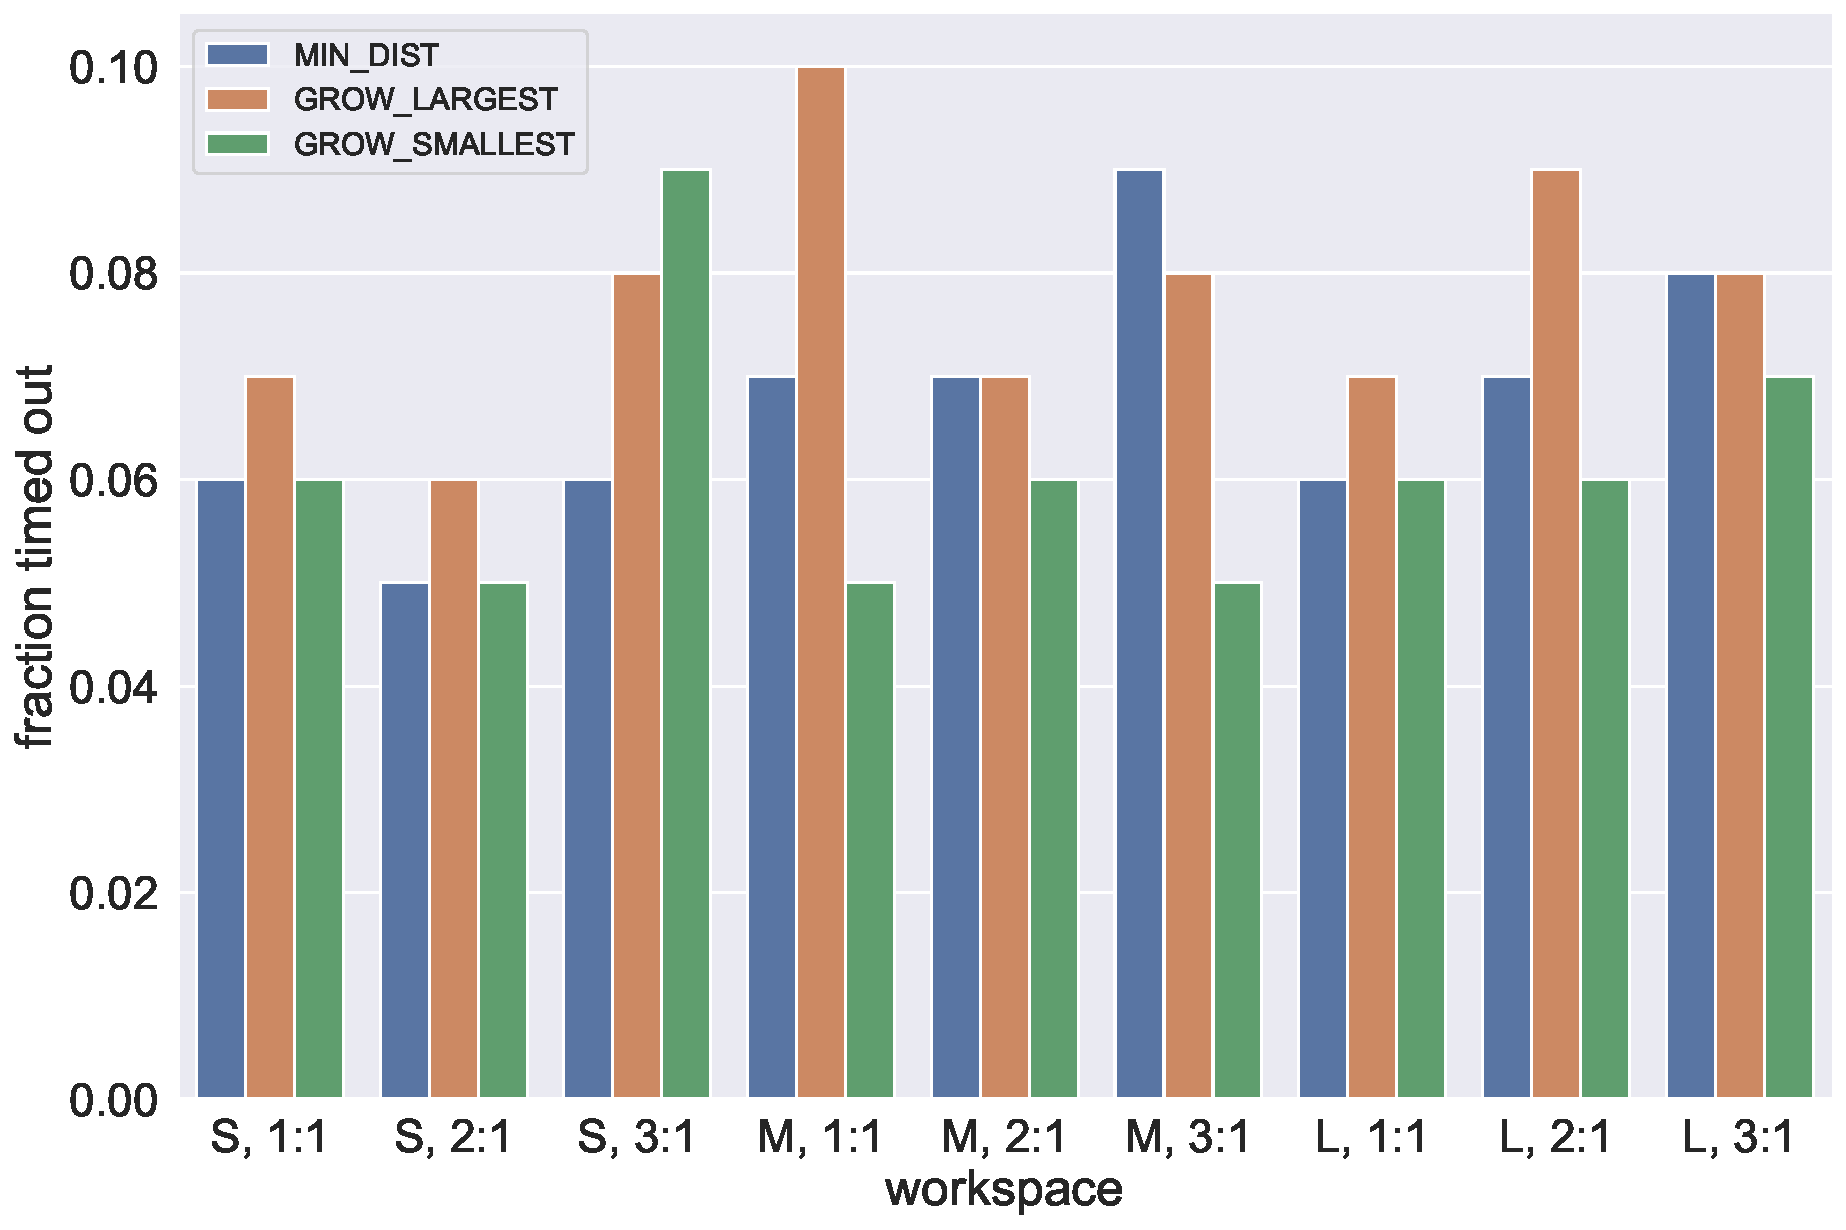
\includegraphics[width=0.9\textwidth]{figures/plots/AFBS_timeout.pdf}
	\caption[]{}
	\label{fig:AFBS_timeout}
\end{figure}

\begin{figure}
	\centering
	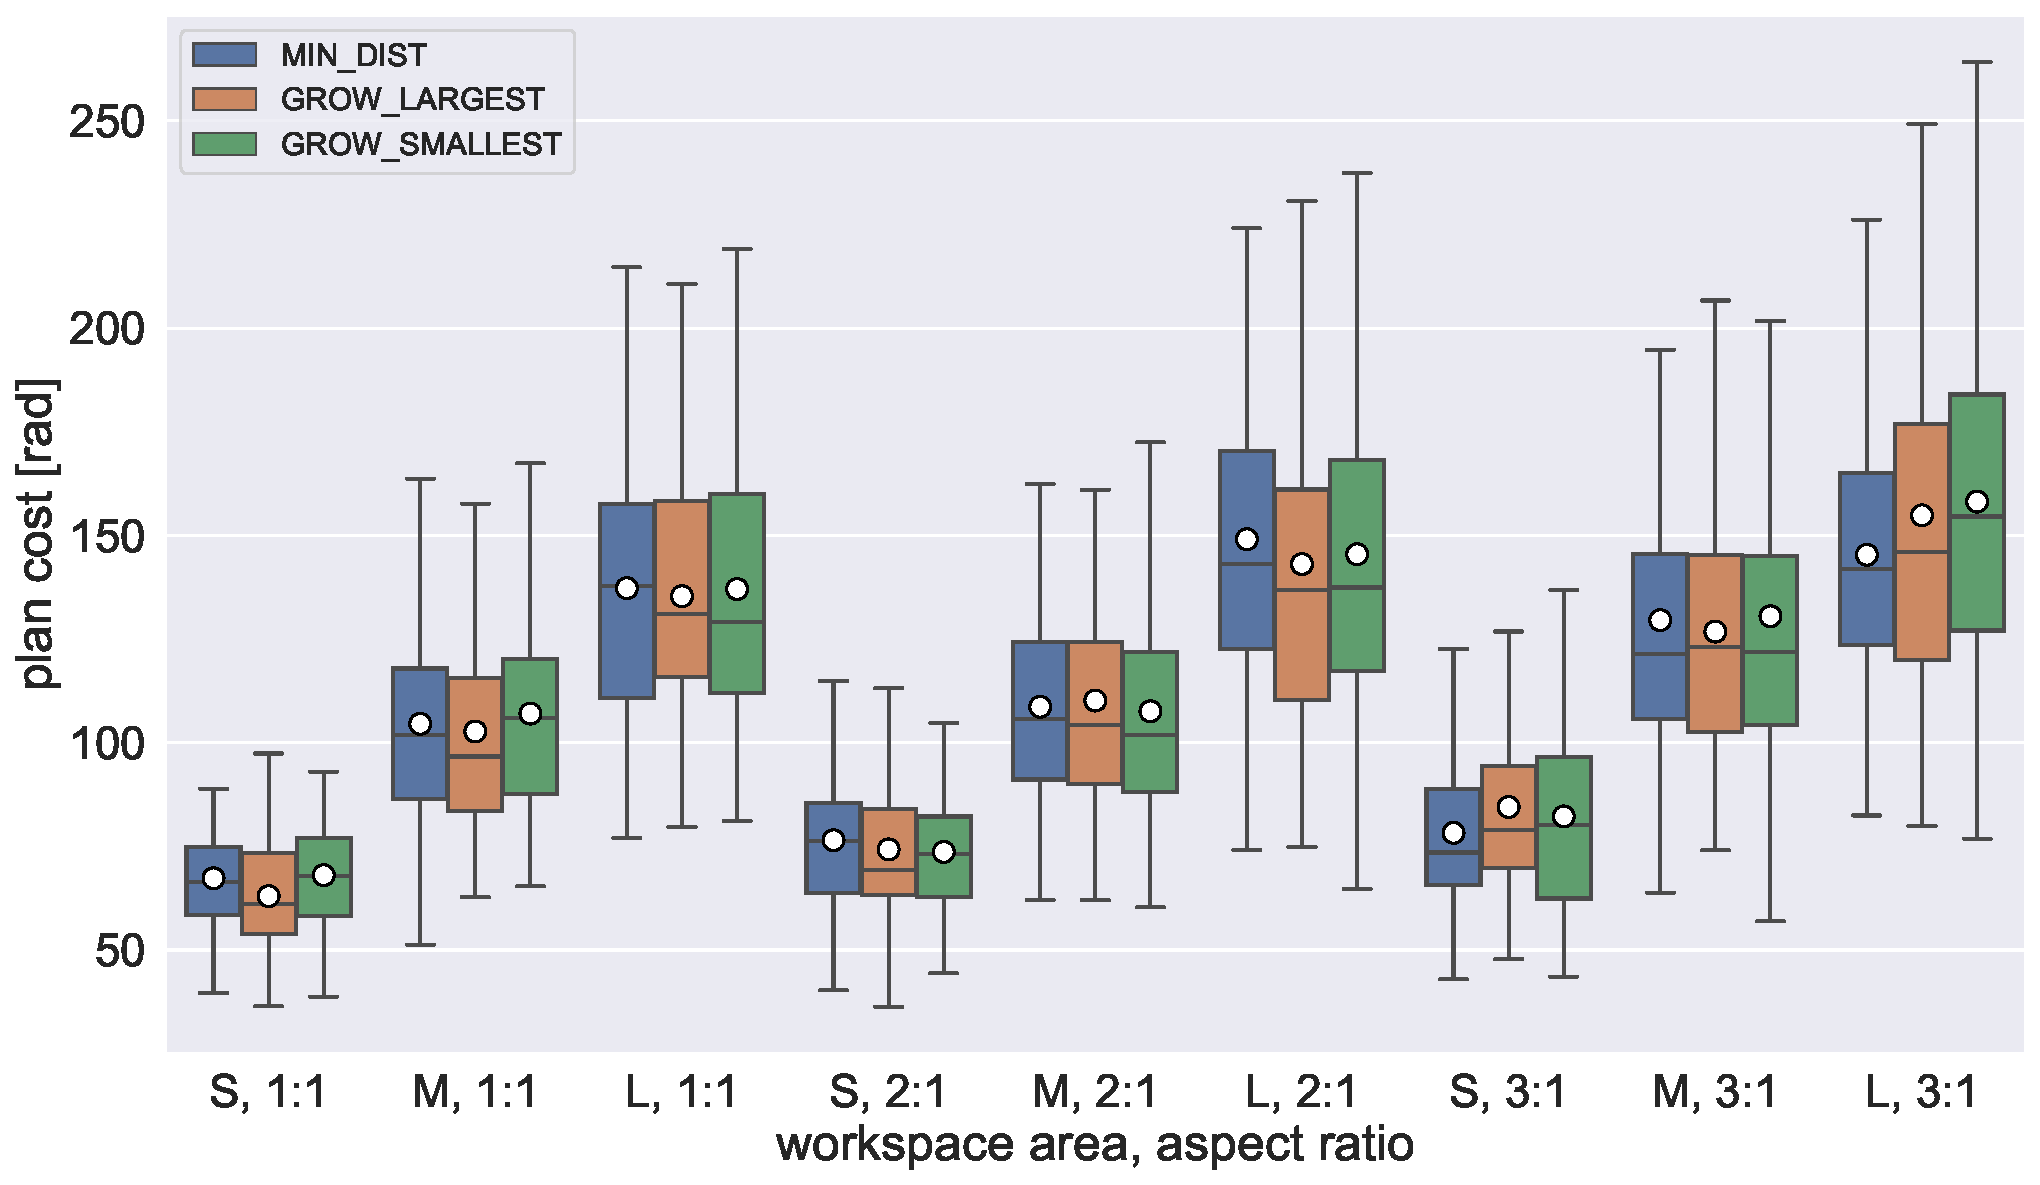
\includegraphics[width=0.9\textwidth]{figures/plots/AFBS_cost.pdf}
	\caption[]{}
	\label{fig:AFBS_cost}
\end{figure}



